\begin{figure*}[t]
\centering
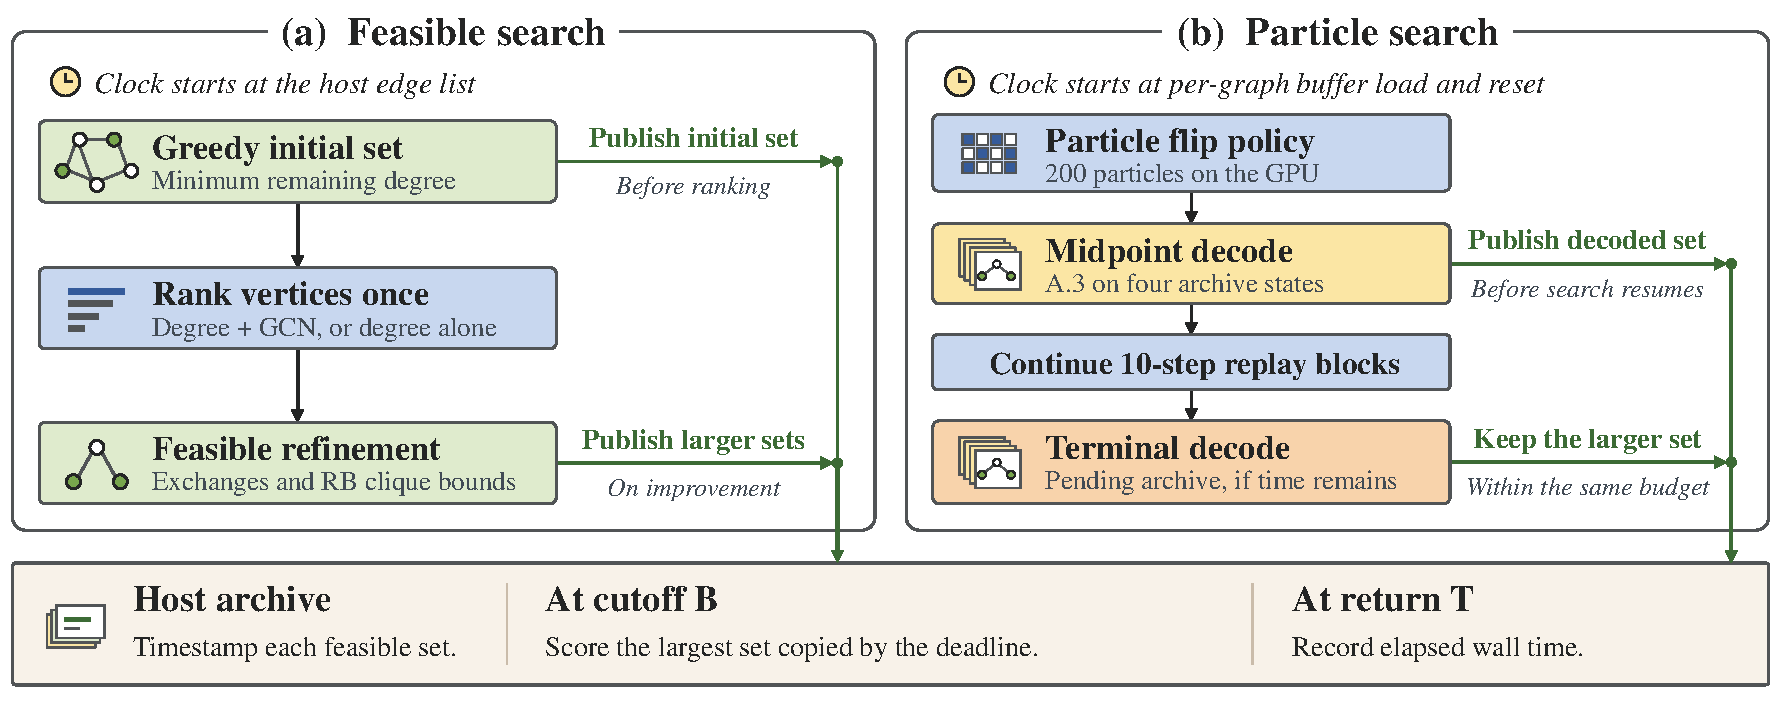
\includegraphics[width=.95\textwidth]{figures/search_paths.pdf}
\caption{\textbf{Two routes to an independent set before the deadline.} Panel titles name the routes: feasible search is SPRINT-C and particle search is SPRINT-S.
Dark arrows show execution order. Green arrows carry feasible vertex sets to the host.
(a) SPRINT-C publishes the greedy set before ranking vertices. The learned and degree-only rankings share the same refinement schedule.
(b) SPRINT-S publishes at the midpoint and again before return. Each readout decodes the four lowest-energy archive entries. Both decodes and their host copies count toward the per-graph budget.
At cutoff \(B\), the host scores the largest set it has received. The solver's return time \(T\) is recorded separately.}
\label{fig:search-paths}
\end{figure*}
